\section{Template Matching}

\emph{What do we want to achieve?}

We want to describe how a succesful match is found for a template when
matching it with an image. We want to explain the main theories behind
the methods, and test our implementation under various circumstances.

\subsection{Main Theory: Use filtering methods}

\subsubsection{Correlation}

All the implementations of template matching (that we use) utilizes
variations of correlation, to compare templates with image segments. The
technique is the same as filtering with various predetermined kernels,
like gaussian, sobel, box-filter etc. , to gain various filter effects,
but instead we use an actual image template as a kernel and measure the
difference between this and a section of the image we want to look
through.

Normal (un-normalized) correlation is mathematically described as:

$h[m,n] = \sum{g[k,i] f[m+k,n+l]}$

Using this method for matching, is prone to a lot of ``false''
positives, as the result is dependent of the actual pixel values, not
determined by the degree of match between the filter and the image
segment. The sum of the multiplied pixel values, will be large in bright
areas of the image and vice versa in the dark areas. To make sure the
correlation also considers the overall brightness of the segment, a
normalized version of the formula is introduced.

If you step out one level of abstraction and view the template H and
image segment F as two vectors (achieved by joining each row or column
after each other), the correlation can be viewed as finding the dot
product between the two vectors. H dot F. (Just take a second and
realize that the dot product is found the same way as we calculate
correlation). As we know a vector can be normalized by dividing it by
its length, we can also normalize the dot product by dividing it by the
multiplication of the length of the two vectors.

the relationship is described in the formula:

$H \cdot F = ||H|| * ||F|| * \cos{V}$

\begin{center} 
$\leftrightarrow$
\end{center}

$\cos{V} = (H \cdot F) /(||H|| * ||F||)$

The normalised expression will always give a result between -1 and 1 as
$\cos{V} \exists [-1,1]$, and since the image vectors only contains
positive numbers the result will be betweem zero and one.

The length of each the two vectors are found with the formula: (here
with a vector in 3 dimensions)

$||a|| = \sqrt{a_1^2 + a_2^2 + a_3^2}$

Translating back from this abstraction level and looking at correlation
again the formula is translated into:

Normalized Cross Correlation:

$(x,y) = \sum{g[k,l] f[m+k,n+l]}$

This can be refined further by subtracting the means for both template
and image patch. This gives us the zero mean normalized
cross-correlation, AKA correlation coefficient:

$h[m,n] = \frac{ \sum{k,l}{(g[k,l]-\bar{g})(f[m+k,n+l]-\bar{f}_{m,n})}}{((\sum{k,l}{g[k,l]-\bar{g})^2\sum{k,l}{(f[m+k,n+l]-\bar{f}_{m,n})^2)}^{0.5}}}$

This gives a very accurate result, but is pretty slow as well.

\textbf{Another implementations using correlation:}

Sum of squared difference:

$(u,v)=\sum{x,y}{f(x,y)-t(x-u,y-v)}^2$

s compares each corresponding pixels describing the difference between
them with a calculated positive number. (because of the squared) The
closer to zero the final result is, the better the match. The image
viewed (where white equals good results) are calculated with: image
(x,y) = 1 - sqrt(result of above expression).

Our Implementation:

\begin{verbatim}
def GetEyeCorners(img, leftTemplate, rightTemplate,pupilPosition=None):
    #The method parameters are: the image, templates and optional pupil position.
    sliderVals = getSliderVals()

    #Enable adjustment from slidervalues for match threshold. 
    matchLeft = cv2.matchTemplate(img,leftTemplate,cv2.TM_CCOEFF_NORMED)
    matchRight = cv2.matchTemplate(img,rightTemplate,cv2.TM_CCOEFF_NORMED)

    #The openCV library allows use of different matching methods. Here we use COOEFF_NORMED = normalized cross corellation.
    #Matching both for left template and right template.

    if (pupilPosition != None):
        #If the pupil position is set, slice the image in two halfs at the pupil position. 
        pupX,pupY = pupilPosition
        matchRight = matchRight[:,pupX:]
        matchLeft = matchLeft[:,:pupX]
    matchListRight = np.nonzero(matchRight > (sliderVals['templateThr']*0.01))
    matchListLeft =  np.nonzero(matchLeft > (sliderVals['templateThr']*0.01))

    #Sort out the results with values below the match threshold.
    matchList = (matchListLeft,matchListRight)
    return matchList
\end{verbatim}
\subsection{Our Results: (Also see video)}

We found that, when using the normalize cross corellation, a good
starting threshold is 0.85. That doesn't draw to many detections from
the start and, provides a good starting point for further adjustments.
All the tests runs utilizes the pupil position, allowing matches for the
left template only in the left side and opposite for the right template
matches.

\subsubsection{Test 1 - Unknown Subject.}

\begin{figure}[htbp]
\centering
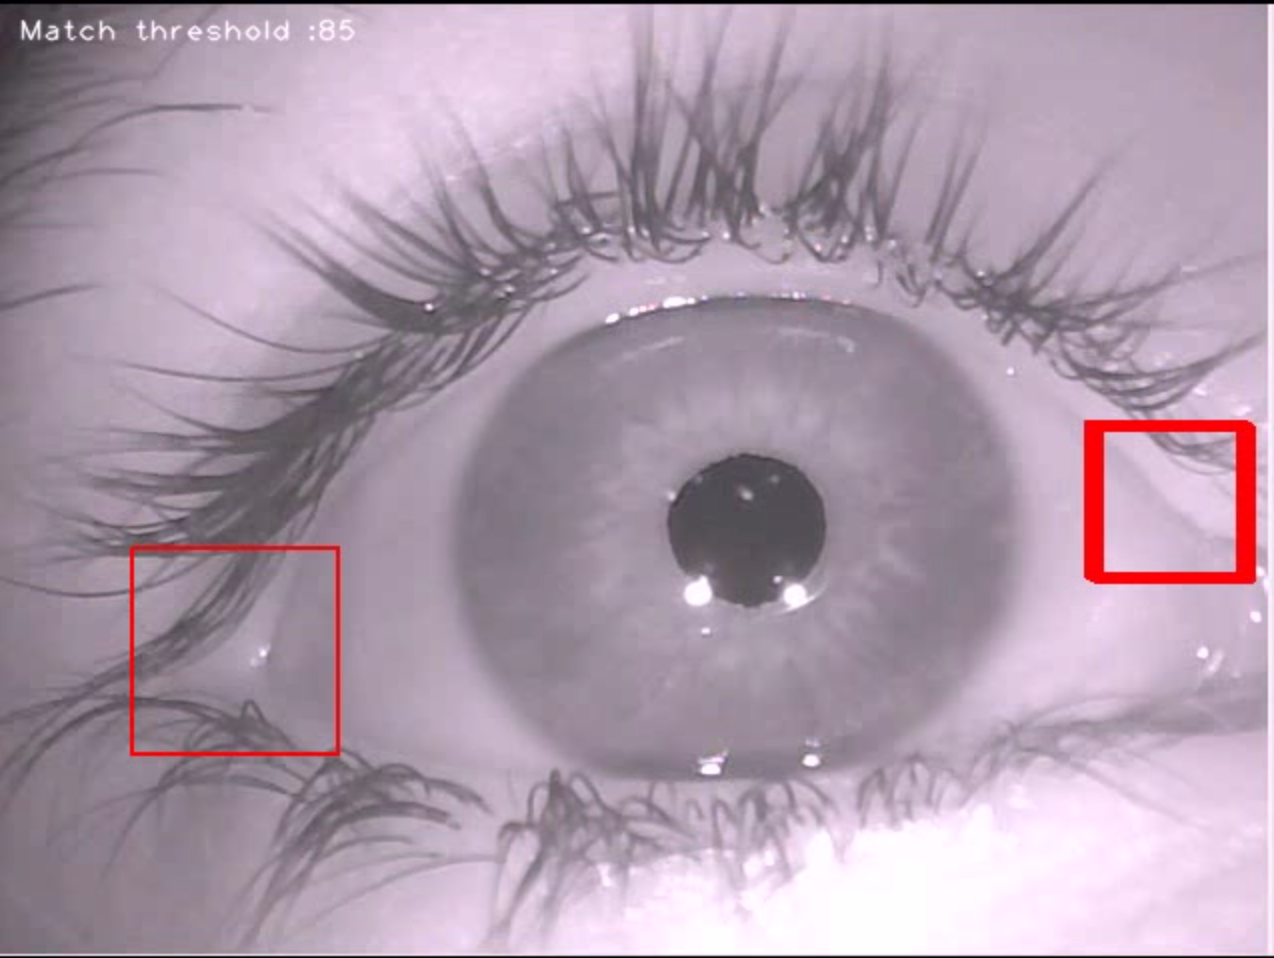
\includegraphics{pics/template_matching/1.png}
\caption{Threshold 85 \label{tm1}}
\end{figure}

As we see in figure \ref{tm1}, with at threshold of 0.85, things work
out fine, when there are not too much movement in the image. In
controlled light, controlled subjects, the correlations methods works
like a charm.

\begin{figure}[htbp]
\centering
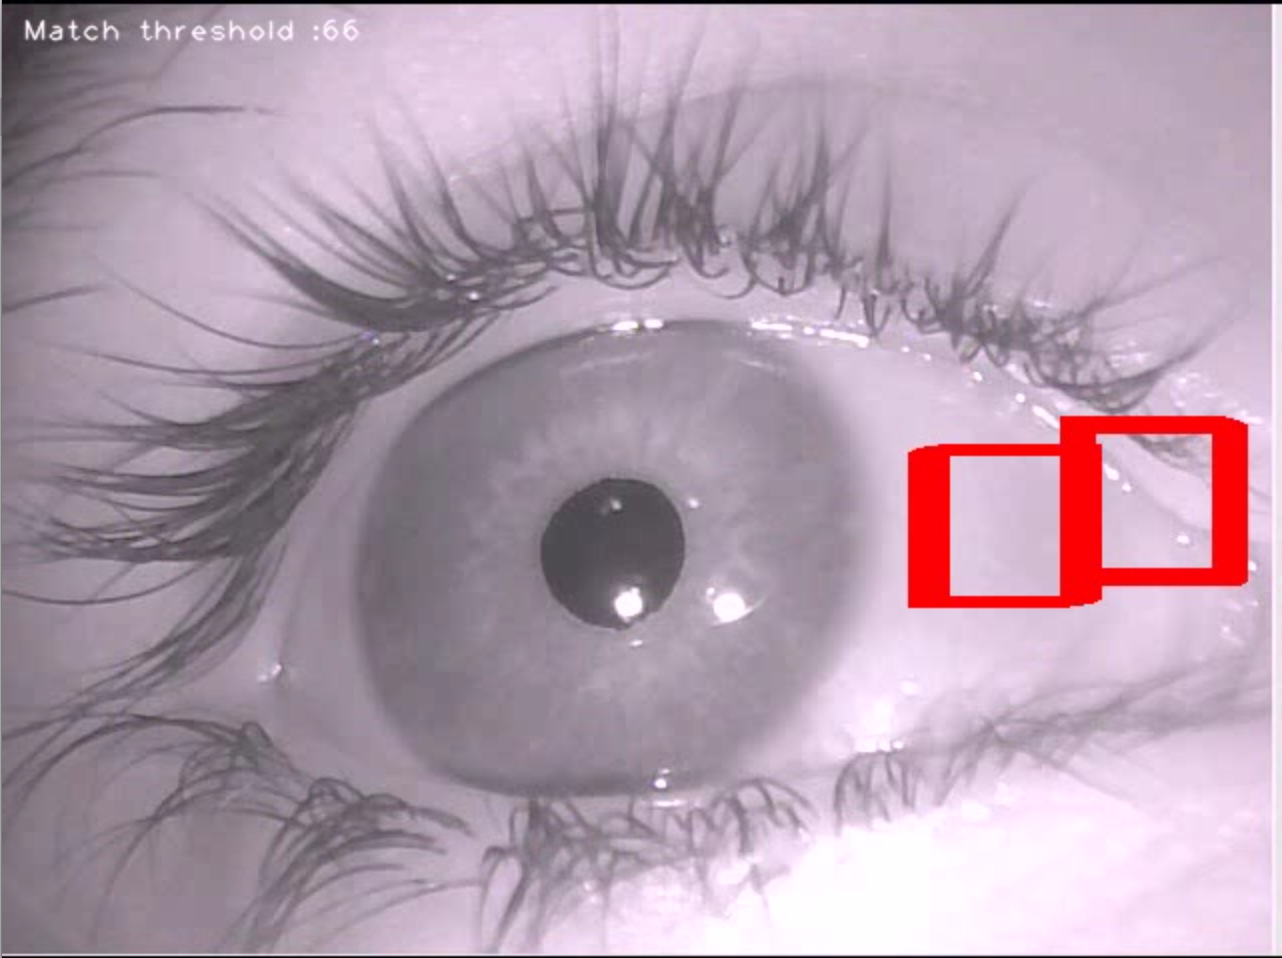
\includegraphics{pics/template_matching/2.png}
\caption{Threshold 66 \label{tm2}}
\end{figure}

Seen in figure \ref{tm2}. As soon as the subject moves too much, the
threshold has to be lowered to find any results. It quickly becomes a
problem having a shared threshold for both template matchings (left \&
right), as the circumstances around the two places in the image are
quite different.

\begin{figure}[htbp]
\centering
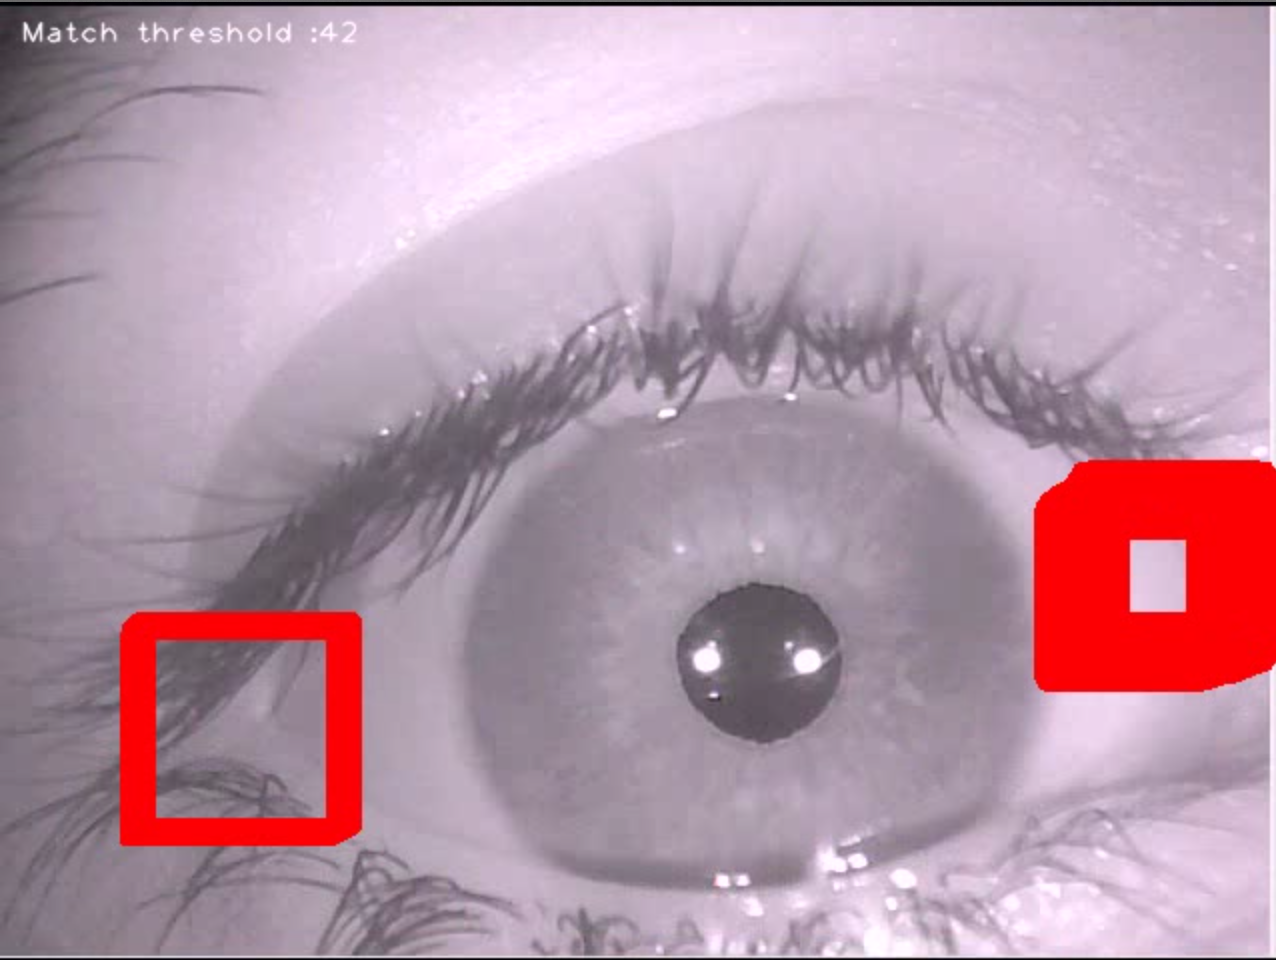
\includegraphics{pics/template_matching/3.png}
\caption{Threshold 42 \label{tm3}}
\end{figure}

Seen in figure \ref{tm3}. Lowering the threshold even more, allows the
subject to move more freely and still finding matches in both sides.
Again we see a big difference in which sides that struggle and which
that finds multible matches.

\subsubsection{Test 2 - Young Master Ghurt - recorded tuesday 12/03/13}

\begin{figure}[htbp]
\centering
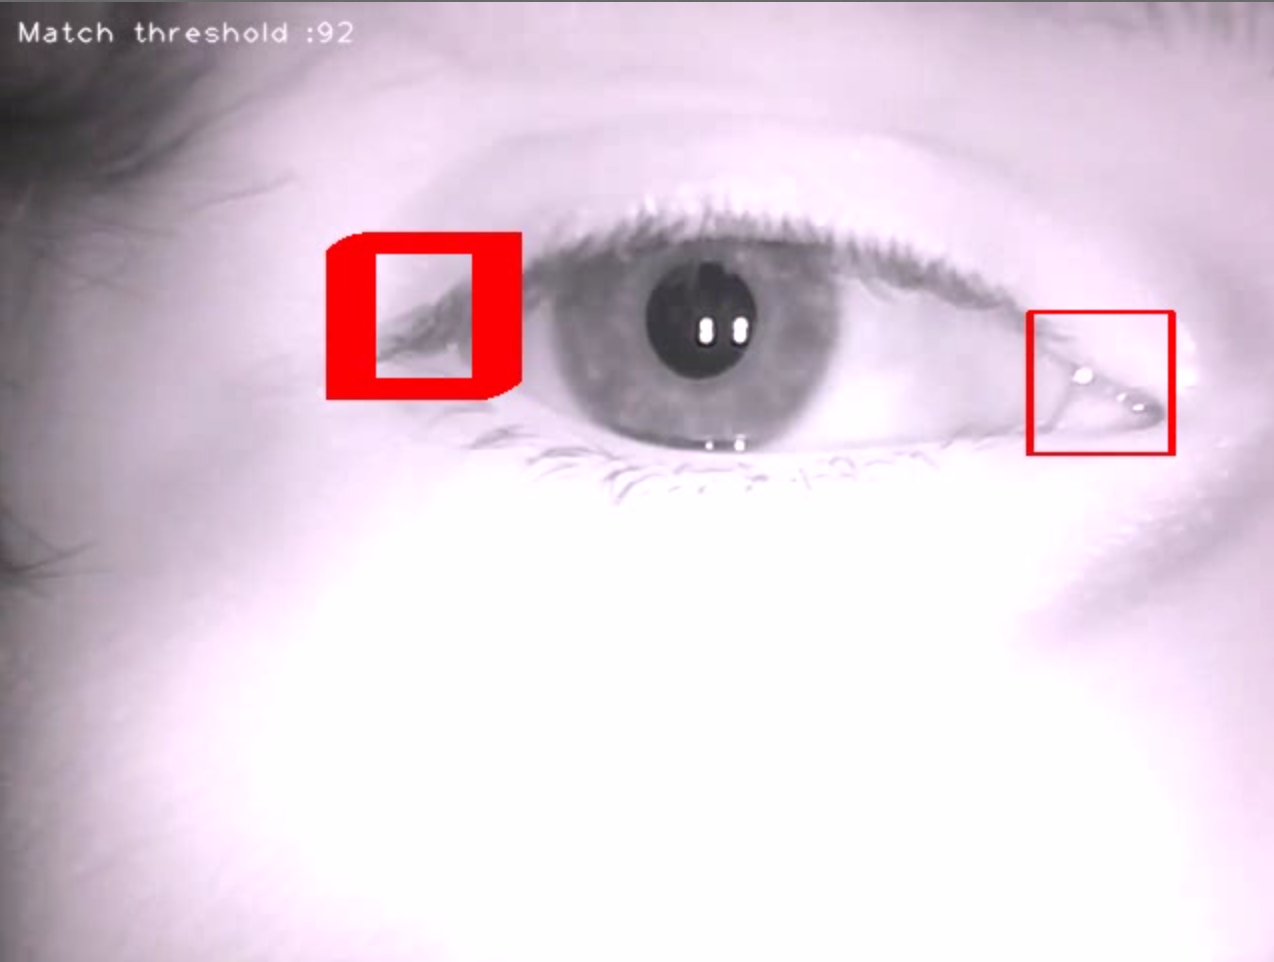
\includegraphics{pics/template_matching/4.png}
\caption{Threshold 92 \label{tm4}}
\end{figure}

In figure \ref{tm4}. Starting out with a high threshold of 0.92 seems to
work quite well. When the template contains enough contrasts/diversity,
and the subject remains still, the errors are few

\begin{figure}[htbp]
\centering
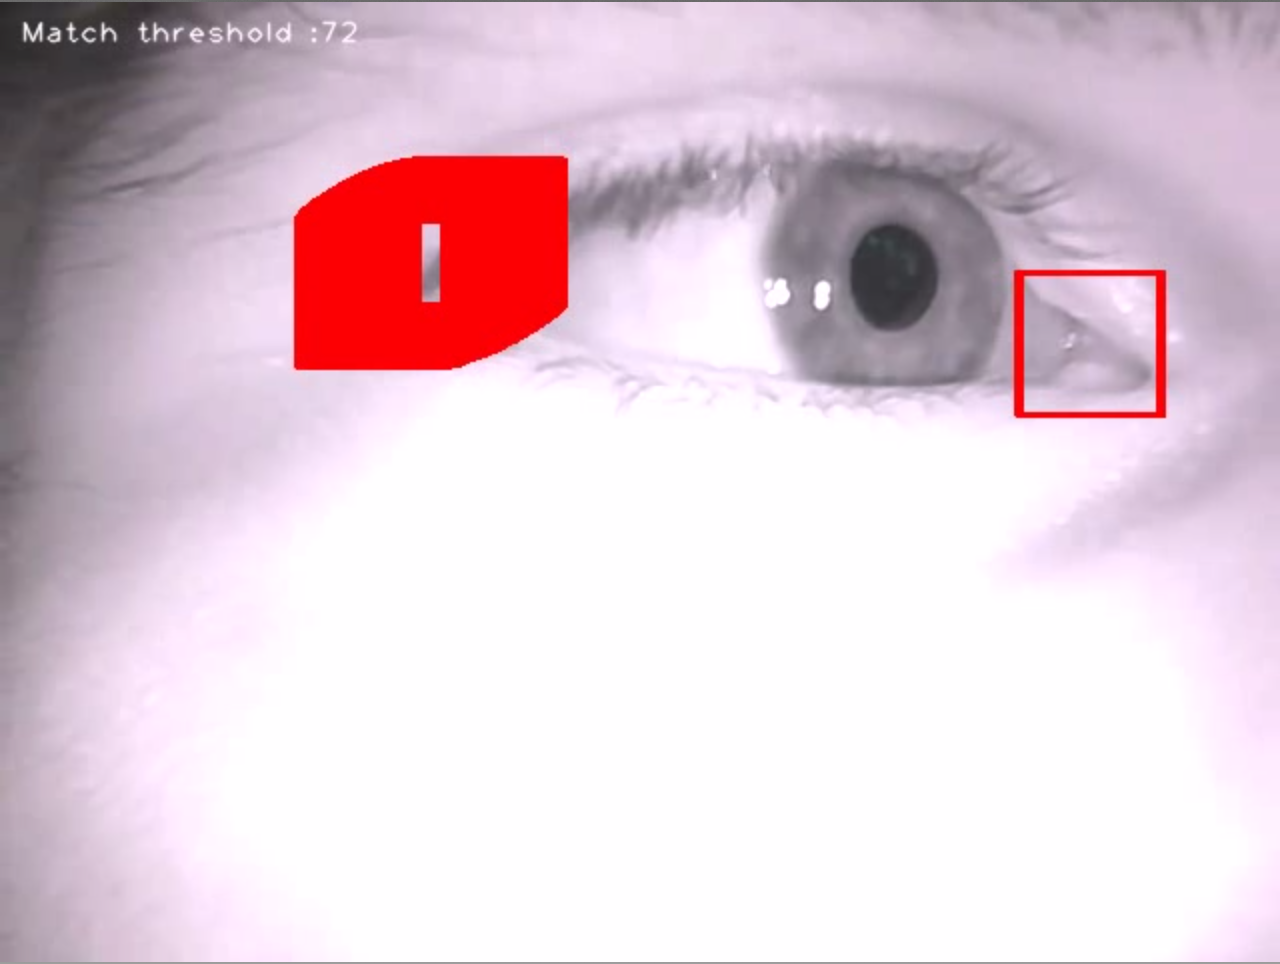
\includegraphics{pics/template_matching/5.png}
\caption{Threshold 72 \label{tm5}}
\end{figure}

In figure \ref{tm5} we see it doesn't take a lot of change before the
threshold has to be lowered to find a result. Again there is a huge
difference on the sides, and we can conclude that a shared threshold
wouldn't be suitable in an industrial/finished solution.

\begin{figure}[htbp]
\centering
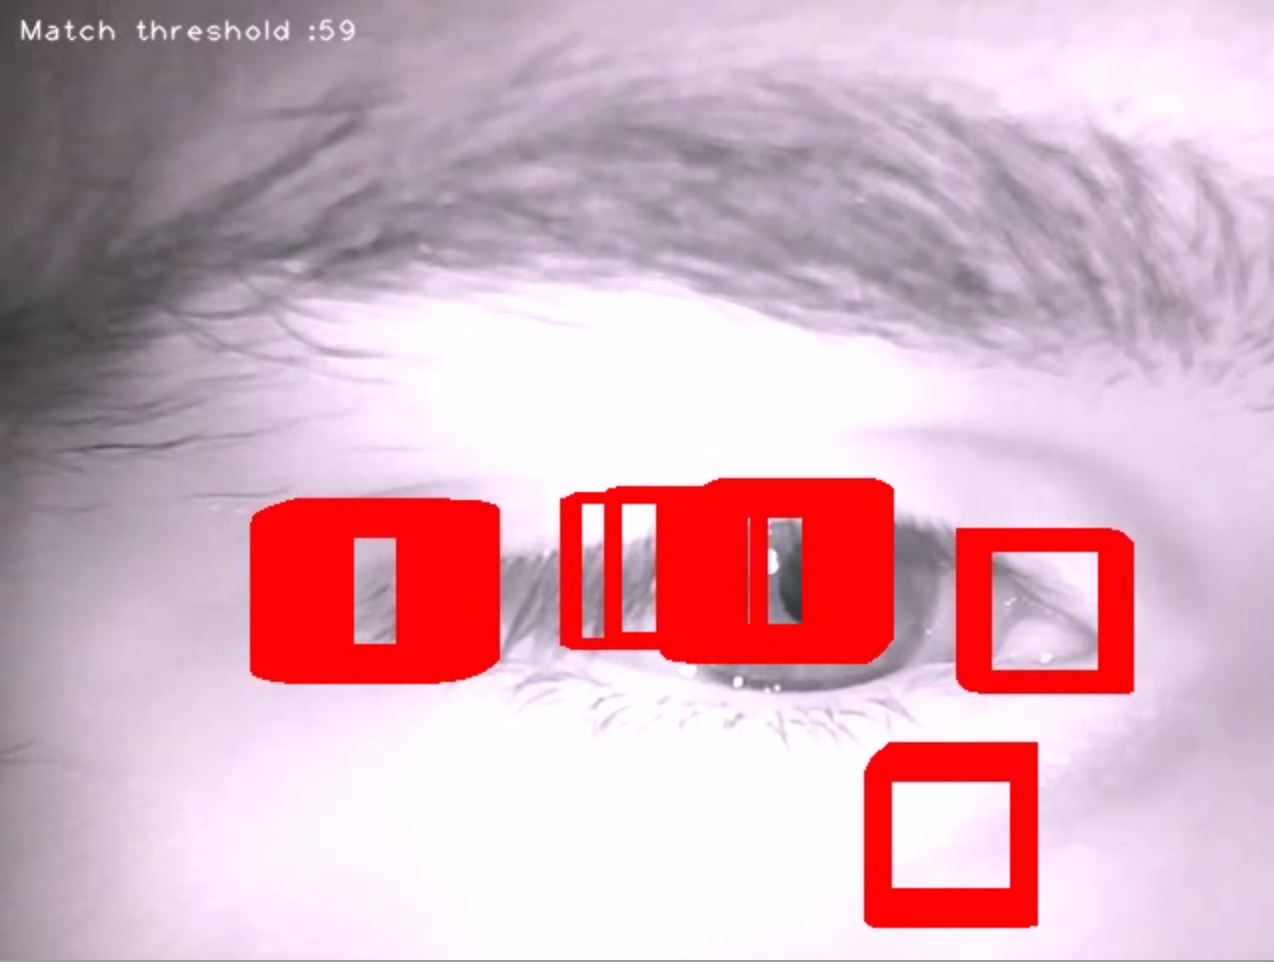
\includegraphics{pics/template_matching/6.png}
\caption{Threshold 59 \label{tm6}}
\end{figure}

In figure \ref{tm6} we see as we continue the path downwards lowering
the threshold to find matches at the sides, a lot of false results now
appear, as the match no longer have to fit perfectly. This is not a bad
setup for further development, as the ``bad'' results easily could be
filtered away. (in the sense that too many matches are better than none
at all).

\subsection{Concluding on the results and improving the method:}

It is obvious that our implementation can be improved. As in all the
different techniques mentioned in this report, controlling the
circumstances are vital for success. Out of the box, cross correlation
proves to be a pretty solid way of finding matches, but it requires the
subject to stand still and keep the same angle towards the camera so the
match area doesn't change completely. The method doesn't provide blazing
speeds as it is now. But this could be improved by performing some of
the work in parallel processes. Instead of matching twice with different
templates, you could use one common template, that would find enough
matches on each side and then filter out bad reslts even more. As of
now, results for are only restricted in that they have to appear on the
correct side of a found pupil location. This could be even more
improved, utilizing the distance from each other, or placement relative
to other facial features. As with the other techniques it proves
impossible to find parameters to fit a sequence of images where the
subject changes/moves. It's far better to find many matches and the
remove ``bad'' results afterwards.
